\documentclass[12pt,a4paper]{article}
\usepackage{tikz}
\usetikzlibrary{arrows}
\usepackage{scalalistings, questions}

% Draw a comparator in the rows given by #1 and #2, with a horizontal
% displacement of #3
\def\comp#1#2#3{%
  \draw (#1)+(#3,0) node {$\bullet$};
  \draw (#2)+(#3,0) node (n2) {$\bullet$};
  \draw[thick] (#1)+(#3,0) -- (n2.center);
}

\def\seq#1{\langle #1 \rangle}

\begin{document}
\begin{center}
\LARGE\bf Concurrent Programming \\
\Large Practical 1: Sorting Networks
\end{center}

This practical builds some networks to sort a list of numbers.  The networks
are not very sensible as software sorting networks; however, they could be
implemented efficiently in hardware.  The main aims of the practical are to
help you get used to thinking about concurrent systems, and to gain familiarity
with the SCL library.

\textbf{Deadline:}  practical sessions in Week~3. 
Your answer should be in the form of well-commented code, answering the
questions below.  You can gain a mark of S by giving decent answers to all the
non-optional questions; you can gain a mark of S+ by giving good answers to
all the questions up to Question~5.  The section marked ``Just for fun'' is
just that.


Each sorting network will be built from \emph{comparators}: simple
two-element sorting components.  A comparator can be pictured as below: 
%
\begin{center}
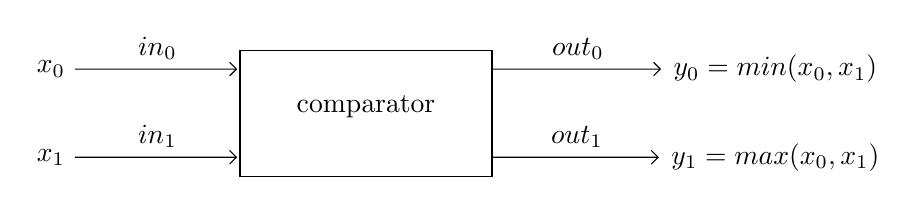
\begin{tikzpicture}[scale = 0.8, >=angle 90,shorten >=1pt]
\node at (0,0.6) {comparator};
\draw (-2,-0.5) rectangle (2,1.5);
\node (x1) at (-5, -0.2) {$x_1$};
\node (x0) at (-5, 1.2) {$x_0$};
\draw[->] (x1) -- node[above]{ $in_1$} (-2,-0.2);
\draw[->] (x0) -- node[above]{ $in_0$} (-2,1.2);
\node (y1) at (6.5,-0.2) {$y_1 = max(x_0,x_1)$};
\node (y0) at (6.5,1.2) {$y_0 = min(x_0,x_1)$};
\draw[->] (2,-0.2) -- node[above]{ $out_1$} (y1);
\draw[->] (2,01.2) -- node[above]{ $out_0$} (y0);
\end{tikzpicture}
\end{center}
%
The comparator has two input channels, $in_0$ and $in_1$, and two output
channels, $out_0$ and $out_1$.  If it inputs $x_0$ and~$x_1$, it outputs their
minimum on~$out_0$ and their maximum on~$out_1$.
\begin{question}
Implement a comparator with the following signature:
%
\begin{scala}
  /** A single comparator, inputting on in0 and in1, and outputting on out0
    * (smaller value) and out1 (larger value). */
  def comparator(in0: ?[Int], in1: ?[Int], out0: ![Int], out1: ![Int]): ThreadGroup
\end{scala}
%
the process should be willing to perform the inputs in either order, and
perform the outputs in either order.  The process should repeat this behaviour
until one of its channels is closed. 
\end{question}

%%%%%

Below is a sorting circuit for four inputs using five comparators.
%
\begin{center}
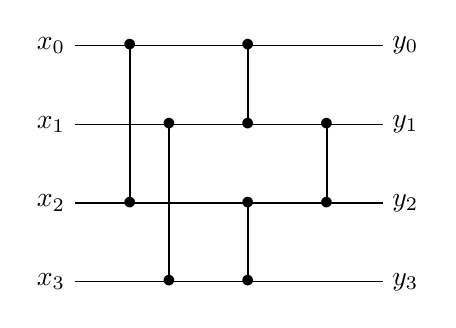
\begin{tikzpicture}
\draw (0,0) node (x0) {$x_0$};
\draw (0,-1) node (x1) {$x_1$};
\draw (0,-2) node (x2) {$x_2$};
\draw (0,-3) node (x3) {$x_3$};
\draw (4.5,0) node (y0) {$y_0$};
\draw (4.5,-1) node (y1) {$y_1$};
\draw (4.5,-2) node (y2) {$y_2$};
\draw (4.5,-3) node (y3) {$y_3$};
\draw (x0) -- (y0);
\draw (x1) -- (y1);
\draw (x2) -- (y2);
\draw (x3) -- (y3);
\comp{x0}{x2}{1}  \comp{x1}{x3}{1.5}
\comp{x0}{x1}{2.5}  \comp{x2}{x3}{2.5}
\comp{x1}{x2}{3.5}
\end{tikzpicture}
\end{center}
%
The first four comparators direct the smallest and largest values to the top
and bottom outputs; the final comparator sorts out the middle two values.
Note that the first two comparators can run concurrently, as can the second
pair: the longest path involves  three comparators.

\begin{question}
\label{Q:sort4}
Implement this sorting circuit, using the following
signature.%% \footnote{The class {\scalashape List} represents lists.  If
  %% you haven't used this class before, you might want to look at the
  %% API documentation, or a relevant on-line tutorial.}
%  
\begin{scala}
  /** A sorting network for four values. */
  def sort4(ins: List[?[Int]], outs: List[![Int]]): ThreadGroup = {
    require(ins.length == 4 && outs.length == 4)
    ...
  }
\end{scala}

Test your implementation using the following idea: pick four random |Ints|,
%% \footnote{%
  %% e.g.~using {\scalashape List.fill(4)(scala.util.Random.nextInt(100))}.}
and send them in on the input channels; receive the outputs and check that
they are a sorted version of the inputs; repeat many times.
%% \footnote{%
  %% You might want to use the {\scalashape sorted} method of the {\scalashape
  %%   List} class.} 
\end{question}

%%%%%

We will now implement a sorting network based on the idea of insertion sort.
%
\begin{question}
\label{Q:insert1}
We want to implement a circuit to insert a value into a sorted list of $n \ge
1$ values, with the following signature.
%
\begin{scala}
  /** Insert a value input on in into a sorted sequence input on ins. 
    * Pre: ins.length = n && outs.length = n+1, for some n >= 1.
    * If the values xs input on ins are sorted, and x is input on in, then a
    * sorted permutation of x::xs is output on ys. */
  def insert(ins: List[?[Int]], in: ?[Int], outs: List[![Int]]): ThreadGroup = {
    val n = ins.length; require(n >= 1 && outs.length == n+1)
    ...
  }
\end{scala}
%
Consider the circuit below to implement |insert| (for $n \ge 2$).  The box
labelled ``$\sm{insert}_{n-1}$'' is (recursively) a circuit to insert the
output of the comparator into the sorted list
$\langle \sm{ins(1)},\ldots,\sm{ins(n-1)} \rangle$ of length~$n-1$.
%
%
\begin{center}
\def\width{6.5} % x coord for output labels
\def\recX{2} % X coord for start of recursive insert
\def\recWidth{3} % width of recursive insert
\def\recEnd{\recX+\recWidth} % X coord of right edge of recursive insert
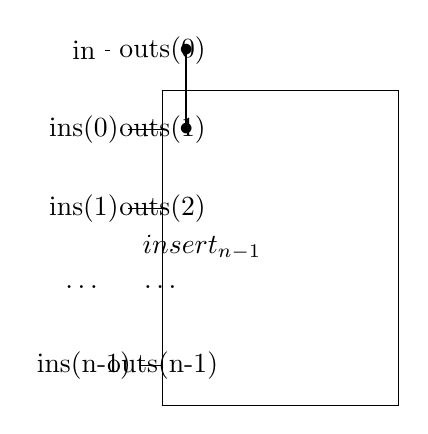
\begin{tikzpicture}
% First row
\draw(0,0) node (in) {\scalashape in};
\draw(\width,0) node (outs0) {\scalashape outs(0)};
\draw (in)--(outs0);
% Recursive insert box
\draw (\recX+1.5,-2.5) node {$\sm{insert}_{n-1}$};
\draw (\recX,-0.5) -- ++(3,0) -- ++ (0,-4) -- ++(-3,0) -- ++ (0,4);
% Second row
\draw (0,-1) node (ins0) {\scalashape ins(0)};
\draw (ins0) -- (\recX,-1);
\comp{in}{ins0}{1.3};
\draw (\width,-1) node (outs1) {\scalashape outs(1)};
\draw (\recEnd,-1) -- (outs1);
%
\draw (0,-2) node (ins1) {\scalashape ins(1)};
\draw (ins1) -- (\recX,-2);
\draw (\width,-2) node (outs2) {\scalashape outs(2)};
\draw (\recEnd,-2) -- (outs2);
%
\draw (0,-3) node {\ldots};
\draw (\width,-3) node {\ldots};
%
\draw (0,-4) node (inslast) {\scalashape ins(n-1)};
\draw (inslast) -- (\recX,-4);
\draw (\width,-4) node (outslast) {\scalashape outs(n-1)};
\draw (\recEnd,-4) -- (outslast);
\end{tikzpicture}
\end{center}
%
Study the circuit and persuade yourself that it indeed implements the
requirements.  Then implement |insert| based upon the circuit.  You will also
need a base case.  Test the circuit.
\end{question}

%%%%%

\begin{question}
\label{Q:insert2}
\textbf{Optional:} The circuit from the previous question had a path
containing $O(n)$ comparators.  Design, implement and test a circuit for
|insert| such that the longest path has length $O(\log n)$.
\end{question}

%%%%%

\begin{question}
Use your function from either Question~\ref{Q:insert1} or~\ref{Q:insert2} to
implement insertion sort.  Use the following signature.
%
\begin{scala}
  /** Insertion sort. */
  def insertionSort(ins: List[?[Int]], outs: List[![Int]]): ThreadGroup = {
    val n = ins.length; require(n >= 2 && outs.length == n)
    ...
  }
\end{scala}
%
You should base your implementation on the following cicuit, where the
sub-circuit $\sm{iSort}_{n-1}$ recursively sorts $n-1$ inputs.

\begin{center}
\def\width{9.5} % x coord for output labels
\def\recStart{1.5} % X coord for start of recursive iSort
\def\recWidth{2.5} % width of recursive iSort
\def\recEnd{\recStart+\recWidth} % X coord of right edge of recursive iSort
\def\insStart{5.5}
\def\insWidth{2.5}
\def\insEnd{\insStart+\insWidth}
%
\begin{tikzpicture}
% Top row
\draw(0,0) node (ins0) {\scalashape ins(0)};
\draw(\width,0) node (outs0) {\scalashape outs(0)};
\draw (ins0)--(\insStart,0); \draw (\insEnd,0)--(outs0);
% Recursive iSort box
\draw (\recStart+1.25,-2.0) node {$\sm{iSort}_{n-1}$};
\draw (\recStart,-0.5) -- ++(\recWidth,0) -- ++(0,-3) -- ++(-\recWidth,0) -- 
  ++(0,3);
% Insert box
\draw (\insStart+1.25,-1.5) node {$\sm{insert}_{n-1}$};
\draw (\insStart,+0.5) -- ++(\insWidth,0) -- ++(0,-4) -- ++(-\insWidth,0) --
  ++(0,4);
% Second row
\draw (0,-1) node (ins1) {\scalashape ins(1)};
\draw (ins1) -- (\recStart,-1);
\draw (\recEnd,-1) -- (\insStart,-1);
\draw (\width,-1) node (outs1) {\scalashape outs(1)};
\draw (\insEnd,-1) -- (outs1);
% Third row
\draw (0,-2) node  {\ldots};
\draw (\recEnd+0.75,-2) node  {\ldots};
\draw(\width,-2) node {\ldots};
% Last row
\draw (0,-3) node (inslast) {\scalashape ins(n-1)};
\draw (inslast) -- (\recStart,-3);
\draw (\recEnd,-3) -- (\insStart,-3);
\draw (\width,-3) node (outslast) {\scalashape outs(n-1)};
\draw (\insEnd,-3) -- (outslast);
\end{tikzpicture}
\end{center}

%
%Again, draw a picture to explain your circuit.

Test your implementation using the ideas from Question~\ref{Q:sort4}.
\end{question}

%%%%%

\subsection*{Just for fun}

Finally, we will implement a technique known as \emph{bitonic
  sorting}.  The idea is closely based on merge sort: small inputs are
sorted directly; larger inputs are split into two; each half is sorted
recursively; and the results are merged together.  For simplicity, we
will assume that the number of inputs is a power of~2.

The merging circuit can be defined recursively.  The base case is
straightforward.  Below is the merging circuit for eight inputs, making use of
two four-input merge circuits and four comparators.  It assumes that the two
halfs of the input, $\seq{x_0,x_1,x_2,x_3}$ and $\seq{x_4,x_5,x_6,x_7}$ are
each sorted, and merges them into a single sorted sequence.
%
\begin{center}
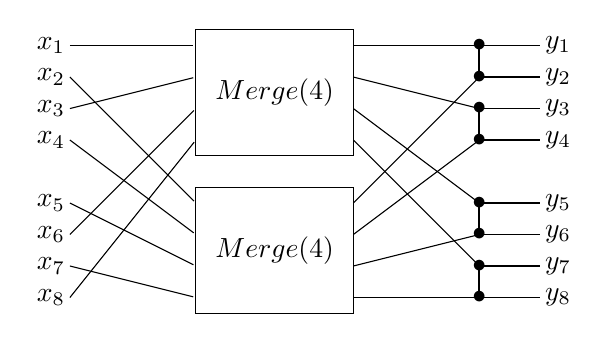
\begin{tikzpicture}[scale = 0.4, >=angle 90,shorten >=1pt]
% input wires
\foreach \y/\i in {4/1,3/2,2/3,1/4,-1/5,-2/6,-3/7,-4/8}
  \node (x\i) at (-0.6,\y){$x_{\i}$};
\foreach \y/\z in {4/4,3/-1,2/3,1/-2,-1/-3,-2/2,-3/-4,-4/1}
  \draw(0,\y) -- (4,\z);
% mergers
\draw(4,-0.5) rectangle (9,-4.5);
\node at (6.5,-2.5) {$Merge(4)$};
\draw(4,0.5) rectangle (9,4.5);
\node at (6.5,2.5) {$Merge(4)$};
% connecting wires
\foreach \y/\z in {4/4, 3/2, 2/-1, 1/-3, -1/3, -2/1, -3/-2, -4/-4}
  \draw(9,\y) -- (13,\z);
% comparators
\foreach \y/\z in {4/3, -1/-2, 2/1, -3/-4}{
  \draw (13,\y) node {$\bullet$};
  \draw (13,\z) node {$\bullet$};
  \draw[thick] (13,\y) -- (13,\z);
}
%\foreach \y in {3.5,1.5,-1.5,-3.5}
  % \draw(13,\y-0.8) rectangle (14,\y+0.8);
%outputs
\foreach \y in {4,3,2,1,-1,-2,-3,-4}
  \draw(13,\y) -- (15,\y);
\foreach \y/\i in {4/1,3/2,2/3,1/4,-1/5,-2/6,-3/7,-4/8}
  \node at (15.5,\y){$y_{\i}$};
\end{tikzpicture}
\end{center}
%
Each half of the input is split between the two sub-merges.  Corresponding
outputs from the two sub-merges are fed into comparators.

\begin{question}
Implement this sorting algorithm.  Use the following signature, for a circuit
for $2^k$ values.
%
\begin{scala}
  /** A merging network for £$2^k$£ values.  If the values received on
    * ins1 and ins2 are sorted, then their merger is output on outs. */
  def merge(k: Int)(ins1: List[?[Int]], ins2: List[?[Int]], outs: List[![Int]])
      : ThreadGroup = {
    val n = 1 << k; val halfN = n/2
    require(k >= 1 && ins1.length == halfN && ins2.length == halfN &&
              outs.length == n)
    ...
  }
\end{scala}
%
You might want to use the following function for doing the splitting.
\begin{scala}
  /** Split xs into two lists, alternately.
    * @return the lists <xs(0), xs(2), xs(4),...> and <xs(1), xs(3), xs(5), ...>
    */
  private def split[T](xs: List[T]): (List[T], List[T]) = 
    if(xs.isEmpty) (List[T](), List[T]())
    else{ val (ys, zs) = split(xs.tail); (xs.head::zs, ys) }
\end{scala}
\end{question}

%%%%%

The sorting circuit itself can also be defined recursively.  The base case is
straightforward.  The recursive case is illustrated below: the input is split
in half; each half is sorted; the results are merged.
% 
\begin{center}
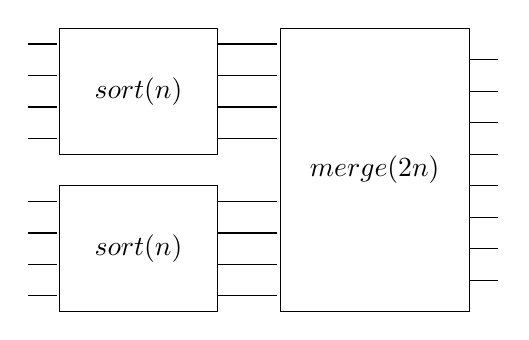
\begin{tikzpicture}[scale = 0.4, >=angle 90,shorten >=1pt]
\foreach \y in {4,3,2,1,-1,-2,-3,-4}
  \draw(0,\y) -- (1,\y);
\draw(1,0.5) rectangle (6,4.5);
\node at (3.5,2.5) {$sort(n)$};
\draw(1,-0.5) rectangle (6,-4.5);
\node at (3.5,-2.5) {$sort(n)$};
\foreach \y in {4,3,2,1,-1,-2,-3,-4}
  \draw(6,\y) -- (8,\y);
\draw(8,-4.5) rectangle (14,4.5);
\node at (11,0){$merge(2n)$};
\foreach \y in {4,3,2,1,0,-1,-2,-3,}
  \draw(14,\y-0.5) -- (15,\y-0.5);
\end{tikzpicture}
\end{center}

\begin{question}
Implement this sorting circuit.  Use the following signature.
%% \footnote{You
  %% might want to use the operations {\scalashape take} and {\scalashape drop}
  %% from the {\scalashape List} class for splitting the input.}
%
\begin{scala}
  /** A bitonic sorting network for 2^k values. */
  def bitonicSort(k: Int)(ins: List[?[Int]], outs: List[![Int]]): ThreadGroup = {
    val n = 1 << k
    require(ins.length == n && outs.length == n)
    ...
  }
\end{scala}

Test your implementation using the ideas from Question~\ref{Q:sort4}.
\end{question}

\end{document}
